%%%%%%%%%%%%%%%%%%%%%%%%%%%%%%%%%%%%%%%%%%%%%%%%%%%%%%%%%%%%%%%
% 10/04/2018
% Esta plantilla fue realizada por los ex alumnos (ahora Ing. Electrónicos) Brignone, Matías Nicolás y Rodríguez, Lucía Fernanda para ser utilizada como modelo para la elaboración del informe final del Proyecto Integrador de la carrera de Ingeniería Electrónica de la Facultad de Ciencias Exactas, Físicas y Naturales (FCEFyN) de la Universidad Nacional de Córdoba (UNC), de acuerdo al estilo sugerido por la cátedra de Proyecto Integrador.

%%%%%%%%%%%%%%%%%%%%%%%%%%%%%%%%%%%%%%%%%%%%%%%%%%%%%%%%%%%%%%%

\documentclass[12pt,A4paper,titlepage, twoside, openright]{report}
% twoside y openright para que el PDF quede listo para ser impreso y encuadernado, garantizando que los capítulos nuevos comiencen siempre del "lado derecho" (agrega páginas en blanco cuando hace falta) y ajustando márgenes internos/externos según sea página par o impar
\raggedbottom

\usepackage[spanish]{babel}
\usepackage[utf8]{inputenc}
\usepackage[T1]{fontenc}
\usepackage{lmodern}
% para manejar la bibliografía, se utiliza biblatex con biber como backend, las entradas bibliográficas se encuentran en el archivo bibliography.bib (deben tener un formato específico, se dejan algunos de ejemplo)
% si no compila correctamente, comentar estas 2 líneas, y comentar también más abajo donde se utiliza \printbibliography, y luego googlear cómo utilizar este paquete (o emplear alguna alternativa)
\usepackage[backend=biber]{biblatex}
\addbibresource{bibliography.bib}
\usepackage{amsmath}
\usepackage{graphicx}
\usepackage{graphicx, wrapfig}
\usepackage{fancyhdr}
\usepackage{anysize}
\usepackage{verbatim}
\usepackage{colortbl}
\usepackage[dvips,final]{epsfig}
\usepackage{float}
\usepackage{textcomp}
%\usepackage{listings} % para incluir código
%\usepackage{minted} % para incluir código, mucho más fácil de personalizar que listings (pero se requiere Python)
\usepackage{blindtext} % para generar texto a los fines de mostrar contenido en el template (se puede eliminar este paquete)
\usepackage{mathabx}
\usepackage{caption}
\usepackage{subcaption}
\usepackage{multirow}
\usepackage{booktabs}
\usepackage{acronym}
\usepackage{emptypage}
\usepackage[titletoc,title]{appendix}
\renewcommand{\tablename}{Tabla}
\usepackage[nottoc]{tocbibind}
\usepackage{pdfpages}
\usepackage{datetime}
\newdateformat{monthyeardate}{%
	\monthname[\THEMONTH] / \THEYEAR}
\makeatletter

\renewcommand{\monthnamespanish}[1][\month]{%
	\@orgargctr=#1\relax
	\ifcase\@orgargctr
	\PackageError{datetime}{Invalid Month number \the\@orgargctr}{%
		Month numbers should go from 1 to 12}%
	\or Enero%
	\or Febrero%
	\or Marzo%
	\or Abril%
	\or Mayo%
	\or Junio%
	\or Julio%
	\or Agosto%
	\or Septiembre%
	\or Octubre%
	\or Noviembre%
	\or Diciembre%
	\else \PackageError{datetime}{Invalid Month number \the\@orgargctr}{%
		Month numbers should go from 1 to 12}%
	\fi}
\makeatother

\usepackage{tabu}
\usepackage[top=2.5cm, bottom=2.5cm, inner=2.0cm, outer=3cm, twoside, marginparwidth=44pt]{geometry}


\usepackage{subfiles} % para incluir archivos de cada capítulo, hay otras alternativas (include o input también sirven)
% si se usa subfiles, los archivo que se importan deben tener el siguiente formato (entre corchetes se pone la ubicación de este archivo (el main)):
%\documentclass[../main.tex]{subfiles}
%\begin{document}
%	...
%\end{document}


\usepackage[hidelinks]{hyperref} % para hacer referencias clickeables (con la opción hidelinks se evita que salga un recuadro muy antiestético), para más personalización con respecto a los colores, usar la opción de abajo
% \usepackage{xcolor}
% \hypersetup{
%     colorlinks,
%     linkcolor={black},
%     citecolor={black},
%     urlcolor={black}
% }

\usepackage{bookmark}

% configura pie de página y encabezado de páginas pares/impares para que quede mejor en la impresión (por ejemplo, el número de página se coloca siempre en la parte externa de la página)
\usepackage{fancyhdr}
\renewcommand{\chaptermark}[1]{\markboth{#1}{}}
\renewcommand{\sectionmark}[1]{\markright{#1}}
\pagestyle{fancy}
\fancyhf{}
\fancyfoot[LE,RO]{\thepage}
\fancyfoot[RE,LO]{Apellido I, Apellido II}
\fancyhead[LO]{\itshape\nouppercase{\rightmark}}
\fancyhead[RE]{\itshape\nouppercase{\leftmark}}
\renewcommand{\footrulewidth}{0.4pt}

% colocar todos los path de las carpetas en las que se guarden las figuras del informe (cuidado con imágenes que tengan igual nombre en carpetas diferentes incluidas aca, se utiliza la primera que se encuentra)
\graphicspath{{figuras/}{ch1_introduccion/figuras/}}

\begin{document}

\renewcommand{\listfigurename}{Lista de Figuras}
\renewcommand{\listtablename}{Lista de Tablas}
\renewcommand{\contentsname}{Índice}

\renewcommand{\tablename}{Tabla}


\newcommand{\HRule}{\rule{\linewidth}{0.5mm}} % Defines a new command for the horizontal lines, change thickness here

\begin{titlepage}
\begin{center}
	
% Logo universidad
\begin{figure}[h]
	\begin{center}
		
\includegraphics{logo_unc.png}
	\end{center}
\end{figure}
\vspace{0.5em}

\textsc{\LARGE Universidad Nacional de Córdoba}\\[0.3cm] % Name of your university/college
\textsc{\Large Facultad de Ciencias Exactas, Físicas y Naturales}\\[0.3cm] % Major heading such as course name
\textsc{\Large Carrera Ingeniería Electrónica}\\[0.75cm] % Minor heading such as course title

\textsc{\large Proyecto integrador para la obtención del título de grado de ingeniero electrónico}\\[1.0cm]

\HRule \\[0.4cm]
\textsc{\textbf{TÍTULO EN MAYÚSCULA}}\\[0.4cm] % título de la tesis
\HRule \\[1.5cm]

% autores
\textsc{\Large Alumnos}\\[0.1cm]
\large \textsc{Apellido}, Nombres y \textsc{Apellido}, Nombres \\[0.5cm]

% directores
\textsc{\large Director}\\[0.1cm]
Ing. \textsc{Apellido}, Nombres \\[0.5cm]

\textsc{\large Co-Director}\\[0.1cm]
Ing. \textsc{Apellido}, Nombres \\[2.5cm]

Córdoba, República Argentina \\
\monthyeardate\today % pone mes y año en el formato correcto de manera automática


\end{center}
\end{titlepage}

\cleardoublepage

\large

% numeracion romana
\pagenumbering{roman}

\cleardoublepage

\chapter*{}
\begin{center}
	
	% Logo universidad
	\begin{figure}[h]
		\begin{center}
			
\includegraphics[scale=0.8]{logo_unc.png}
		\end{center}
	\end{figure}
	\vspace{0.25em}
	
	\textsc{\LARGE Universidad Nacional de Córdoba}\\[0.3cm] % Name of your university/college
	\textsc{\large Facultad de Ciencias Exactas, Físicas y Naturales}\\[0.3cm] % Major heading such as course name
	\textsc{\large Escuela de Ingeniería Electrónica}\\[0.75cm] % Minor heading such as course title
\end{center}

El Tribunal Evaluador reunido en este acto y luego de haber aprobado la Solicitud de Aprobación de Tema y efectuado las distintas instancias de correcciones del Informe del Proyecto Integrador para la obtención del Título de Grado “Ingeniero Electrónico” y cumpliendo con el Reglamento correspondiente, declaran el Informe Final de los estudiantes \textbf{Apellido, Nombres} y \textbf{Apellido, Nombres} como “aceptado sin correcciones” y la defensa oral Aprobada. Por lo tanto, luego de haber tenido en cuenta los aspectos de evaluación que indica el Reglamento, el Proyecto Integrador se considera Aprobado.
\\
\\
Se firma el Acta de Examen correspondiente y se distribuyen los ejemplares impresos.
\\
\\
\\
\\
\\
\\
Firma y aclaración del Tribunal Evaluador
\\
\\
Fecha:

\chapter*{Dedicatoria}
\addcontentsline{toc}{chapter}{Dedicatoria}

\begin{flushright}
	\textit{Para nuestras familias...}
\end{flushright}


\chapter*{Agradecimientos}
\addcontentsline{toc}{chapter}{Agradecimientos} 

\textit{A nuestros padres, madres y hermanos, por su incondicional apoyo a lo largo de toda la carrera.}
\\

\textit{A nuestros directores, Apellido Nombre y Apellido Nombre, por la excelente predisposición, la confianza y todo el soporte brindado que hizo posible este proyecto.}
\\

\textit{A nuestros amigos y futuros colegas, quienes hicieron de estos años de estudio una experiencia más placentera.}
\\

\textit{A -Lugar donde se realizó el PI-, junto a todo su personal, por las oportunidades y enseñanzas compartidas.}
\\

\textit{A la Facultad de Ciencias Exactas, Físicas y Naturales de la Universidad Nacional de Córdoba, por la oportunidad de realizar esta carrera de grado.}


\chapter*{Resumen}
\addcontentsline{toc}{chapter}{Resumen}

En este trabajo...
\\
\\

\textbf{Áreas Temáticas del Proyecto Integrador}: 

\textbf{Asignaturas}: 

\textbf{Palabras Claves}:

\chapter*{Abstract}

In this thesis...
\\
\\
\textbf{Key Words}: 


\tableofcontents % arma el índice 
\listoftables % arma la lista de tablas
\listoffigures % arma la lista de figuras


\chapter*{Lista de Acrónimos}
\markboth{Lista de Acrónimos}{}
\addcontentsline{toc}{chapter}{Lista de Acrónimos}
\subfile{acronimos.tex} % colocar en este archivo todos los acronimos, debe tener el siguiente formato el archivo:
%\begin{document}
%	\begin{acronym}
%		\acro{SAT}{Solicitud de Aprobación de Tema}
%	\end{acronym}
%\end{document}

\clearpage	

% numeracion arabic ("normal")
\pagenumbering{arabic}
 
% LA IDEA ES MANTENER CADA CAPITULO EN UN ARCHIVO .tex SEPARADO
% Se deja el capítulo de introducción a modo de ejemplo 
 
\chapter{Introducción}
\label{ch:intro}
\subfile{ch1_introduccion/introduccion.tex}

 
\part{Marco Teórico}
	\chapter{Nombre Capítulo A}
	\label{ch:nombre_capitulo_a}
%	\subfile{chA_nombre_capitulo_a/nombre_capitulo_a.tex}
	
	\chapter{Nombre Capítulo B}
	\label{ch:nombre_capitulo_b}
%	\subfile{chB_nombre_capitulo_b/nombre_capitulo_a.tex}

\part{Marco Metodológico}
	\chapter{Nombre Capítulo C}
	\label{ch:nombre_capitulo_c}
%	\subfile{chC_nombre_capitulo_c/nombre_capitulo_c.tex}

	\chapter{Nombre Capítulo D}
	\label{ch:nombre_capitulo_d}
%	\subfile{chD_nombre_capitulo_d/nombre_capitulo_d.tex}
	
	\chapter{Resultados}
	\label{ch:resultados}
%	\subfile{chE_resultados/resultados.tex}

\bookmarksetup{startatroot}

\chapter{Conclusiones}
\label{ch:conclusiones}
%\subfile{chF_conclusiones/conclusiones.tex}

% se imprimi toda la bibliografia, independientemente de si ha sido citada o no
\nocite{*}
\printbibliography[heading=bibintoc, title={Bibliografía}]


% apéndices/anexos
\appendix
\chapter{Nombre Apéndice I}
\label{app:apendice_I}
%\subfile{apendices/ap_uno.tex}

\chapter{Anexos del Proyecto Integrador}

\section{Solicitud de Aprobación de Tema}
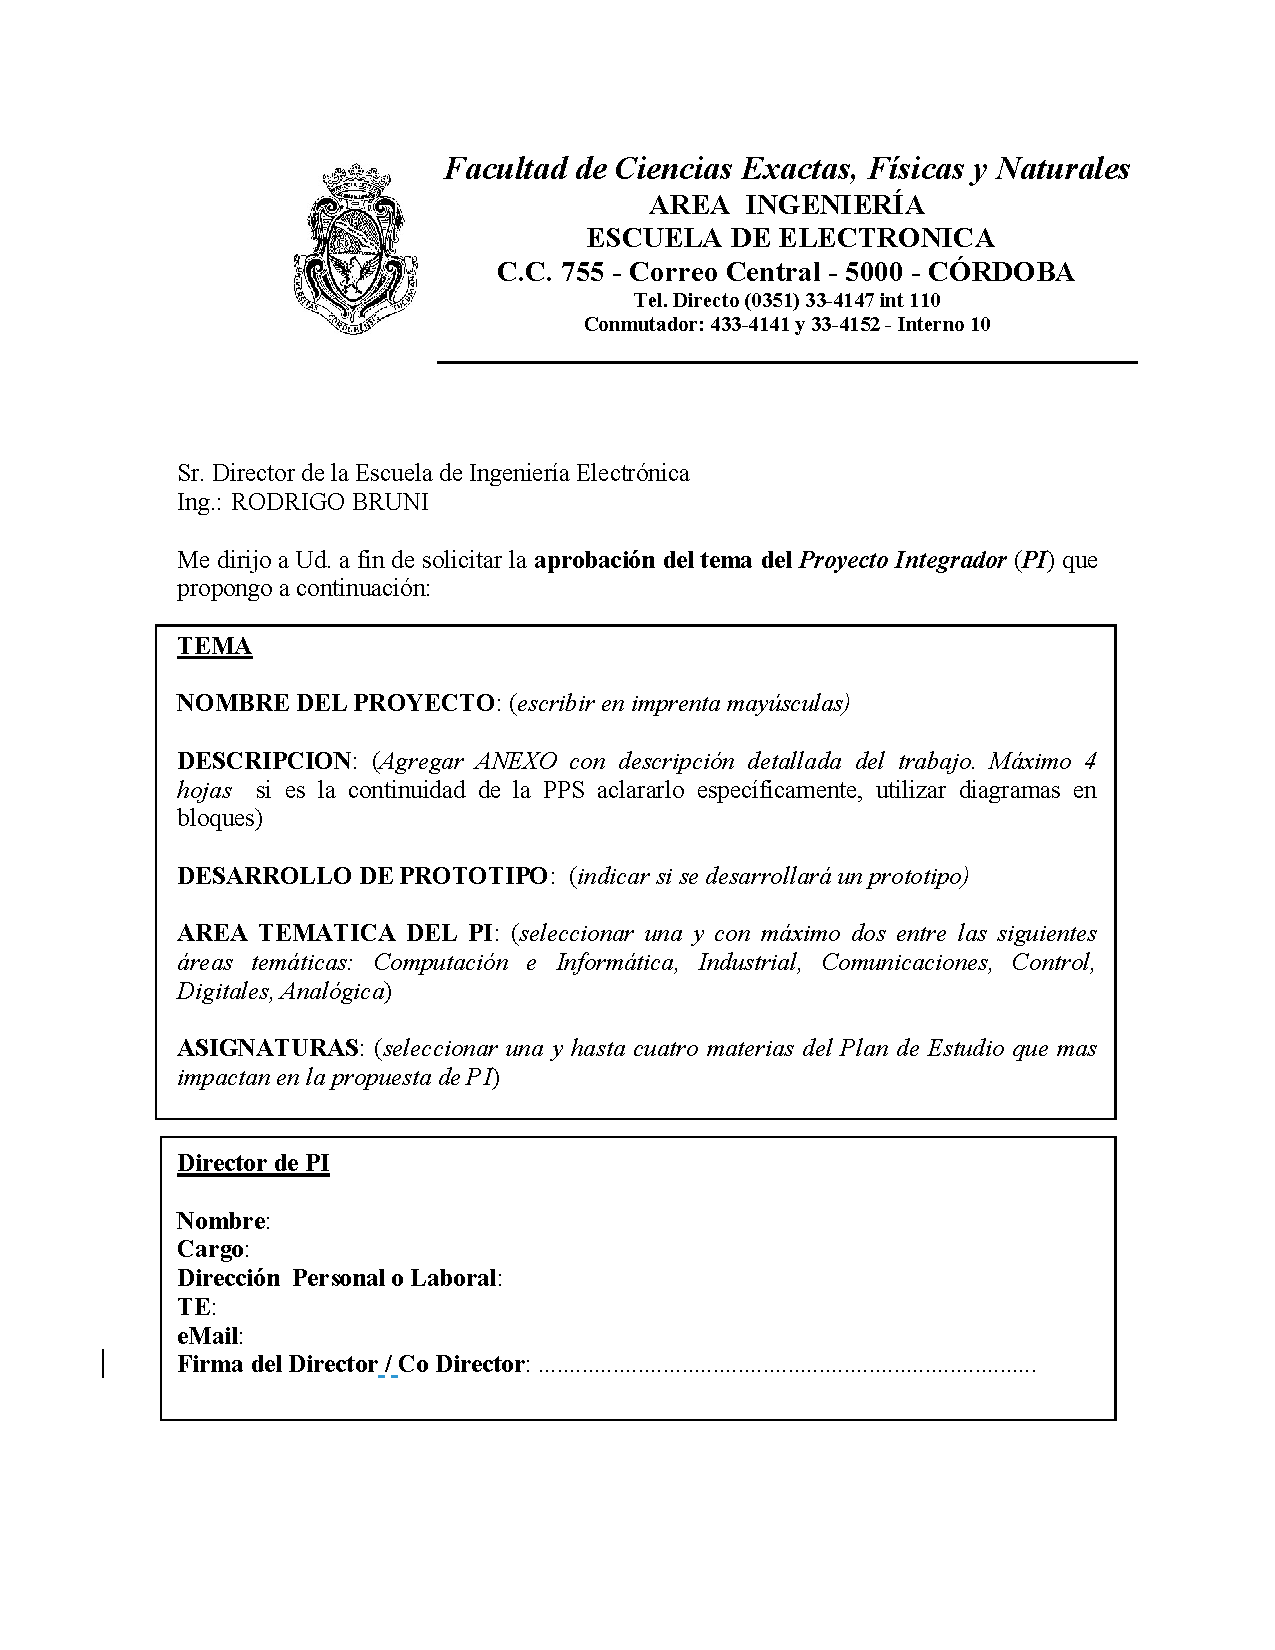
\includepdf[pages=-, pagecommand={}]{sat} % se incluye directamente el PDF de la SAT, el informe sigue con sus encabezados/pies de página/numeración normal

% Se colocan los diferentes informes de avances mensuales enviados a la cátedra, también se incluye directamente el PDF

\includepdf[offset=0 -1cm, pages=-, pagecommand={\section{Informes Mensuales}}]{avance_mensual_1}


\includepdf[pages=-, pagecommand={}]{avance_mensual_2}

\newpage
%\chapter*{}
\begin{center}
	
	% Logo universidad
	\begin{figure}[h]
		\begin{center}
			
\includegraphics[scale=0.8]{logo_unc.png}
		\end{center}
	\end{figure}
	\vspace{0.25em}
	
	\textsc{\LARGE Universidad Nacional de Córdoba}\\[0.3cm] % Name of your university/college
	\textsc{\large Facultad de Ciencias Exactas, Físicas y Naturales}\\[0.3cm] % Major heading such as course name
	\textsc{\large Escuela de Ingeniería Electrónica}\\[0.75cm] % Minor heading such as course title
\end{center}

Quien suscribe el Profesor Apellido, Nombres en su carácter de Director del Proyecto Integrador de los Estudiantes Apellido, Nombres y Apellido, Nombres, denominado: TÍTULO EN MAYÚSCULA, considera que el desarrollo del trabajo se ha completado según lo especificado en la Solicitud de Aprobación de Tema y se encuentra en condiciones de tramitar su defensa.
\\

A los efectos de quien corresponda, en fecha ...../...../2018.
\\
\\
\\
\\
\\
\\
\\
\\
\\

\begin{flushright}
Firma y aclaración del Director
\end{flushright} 


\end{document}